\documentclass[12pt]{article}

\usepackage[utf8]{inputenc}
\usepackage{latexsym,amsfonts,amssymb,amsthm,amsmath, graphicx, float}

\setlength{\parindent}{0in}
\setlength{\oddsidemargin}{0in}
\setlength{\textwidth}{6.5in}
\setlength{\textheight}{8.8in}
\setlength{\topmargin}{0in}
\setlength{\headheight}{18pt}



\title{Assignment 1 — Applied Algorithms, T. II/2024–25}
\author{Austin Jetrin Maddison 6481268}

\begin{document}
	
	\maketitle
	
	\vspace{0.5in}
	
	\subsection*{Problem 1. Las Vegas and Monte Carlo}
	
	
	a.i) We want to show the probablity of running time of Monte Carlo is atleast the worst running time which is $4f(n)$. We can use markov inqualities to bound it..
	\\

	\begin{align*}
		\textbf{P}(X \le \lambda ) & \le \frac{ E [ X ] }{ \lambda }\\
	\end{align*}

	\begin{align*}
		\textbf{P}(T(n) \le 4f(n) ) & \le \frac{f(n)}{4f(n)}\\
								    & \le \frac{1}{4}		
	\end{align*}
	
	a.ii) The worse-case running time happens at most 1/4 which produces incorrect answers. We can get the complement of the last answer...    

	\begin{align*}
		1 - \textbf{P}(T(n) \le 4f(n) ) &  \le 1 - \frac{1}{4} = \frac{3}{4}
	\end{align*}
	
	b.i) The LV algorithm running time is described as the follwing. Each iteration requires running A to produce an answer then run C to check the answer. So the running time for each trial is...
	
	\begin{align*}
		\text{1 iteration running time of LV} = f(n) + g(n)
	\end{align*}

	So the question is what is the expected iterations needed to run LV to get a correct answer. If p is the probablity of success then the expected $1/p$.

	\begin{align*}
		\text{Running time of LV} = \frac{1}{p}(f(n) + g(n))
	\end{align*}

	\vspace{2in} %Leave space for comments!
	
	
	\subsection*{Problem 2. Chernoff-Hoeffding With Bounds}
	(Statement of problem goes here.)\\

	\begin{align*}
		\mathrm{Pr}[X > (1+\varepsilon)\mu H]\leq\exp\left(-\frac{\varepsilon^{2}}{2+\varepsilon}\mu H\right)
	\end{align*}
	
	\begin{proof}
		(Type your proof here.)
	\end{proof}
	
	\vspace{2in} %Leave space for comments!
	
	
	\subsection*{Problem 3. Rescaling Trick}
	(Statement of problem goes here.)\\
	
	\begin{proof}
		(Type your proof here.)
	\end{proof}
	
	\vspace{2in} %Leave space for comments!
	
	
	
	\subsection*{Problem 4. $x^2$ With $\pi$ Degrees of Freedom}
	(Statement of problem goes here.)\\
	
	\begin{proof}
		(Type your proof here.)
	\end{proof}
	
	\vspace{2in} %Leave space for comments!
	
	
	\subsection*{Problem 5. Simple Samplers.}
	(Statement of problem goes here.)\\
	
	\begin{proof}
		(Type your proof here.)
	\end{proof}
	
	\vspace{2in} %Leave space for comments!
	
	
	\subsection*{Problem 6. Median of Means}
	(Statement of problem goes here.)\\
	
	\begin{proof}
		(Type your proof here.)
	\end{proof}
	
	\vspace{2in} %Leave space for comments!
	
	
	\subsection*{Problem 7. Skip List}
	
	a.) Questions to experiment:\\
	
	Q1.) Can we compute count coin tosses differently and is the alternative better?
	
	Q2.) How does varying max height change performance?
	
	Q3.) Linked lists are known to be cache unfriendly, is there a way we can modify 
	
	Q3.) How does it perform against a reputable ordered map?
	\\\\
	
	b.) Search algorithm of Skip List when start is at the bottom left corner in $O(\log(d))$ where d is the number of elements smaller than the key?
	

	
	\vspace{2in} %Leave space for comments!
	
	
	
	\subsection*{Problem 8. ($a,b$) tree. ($2, 3$) tree.}

	a.)	
	\begin{figure}[H] 
		\centering
		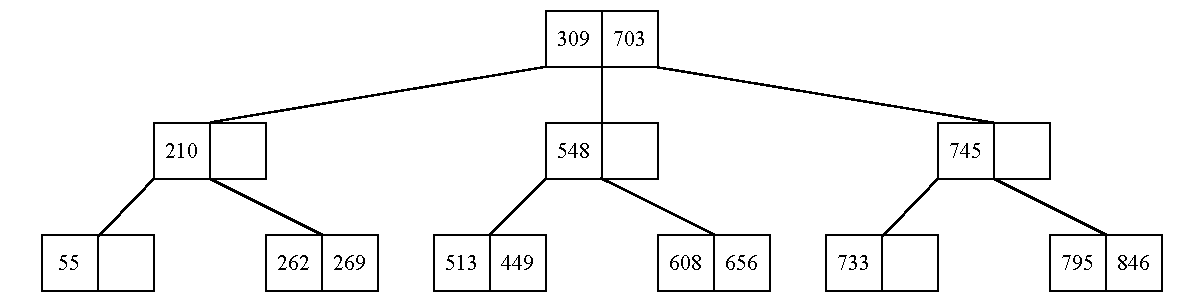
\includegraphics[width=0.9\linewidth]{Q8_a.drawio}
		\caption{Keys $733, 703, 608, 846, 309, 269, 55, 745, 548, 449, 513, 210, 795, 656, 262$ inserted into a $(2, 3)$ tree.}
		\label{fig:q8a}
	\end{figure}
	

	
	b.) 
	\begin{figure}[H] 
		\centering
		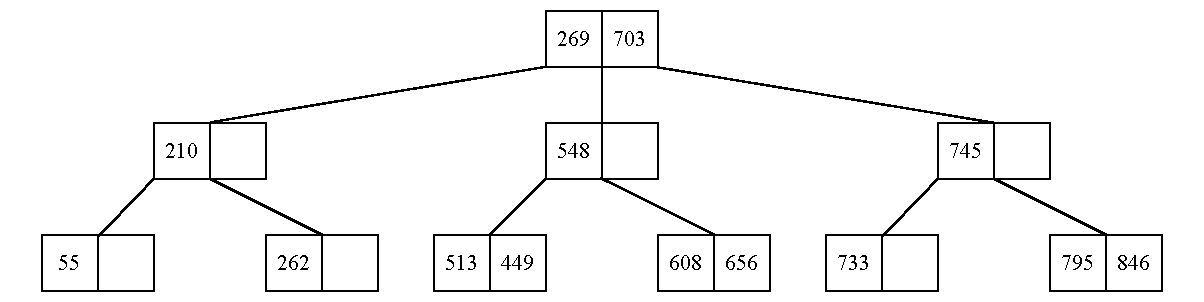
\includegraphics[width=0.9\linewidth]{Q8_b.drawio}
		\caption{Key 309 removed from Figure~\ref{fig:q8a} tree.}
		\label{fig:q8b}
	\end{figure}
	
	
	\vspace{2in} %Leave space for comments!
	
	
	\subsection*{Problem 9. B-Tree Speed}
	(Statement of problem goes here.)\\
	
	\begin{proof}
		(Type your proof here.)
	\end{proof}
	
	\vspace{2in} %Leave more space for comments!
	
	
	
	
	
\end{document}